\documentclass[a4paper,14pt]{extreport} % формат документа

\usepackage{amsmath}
\usepackage{cmap} % поиск в ПДФ
\usepackage[T2A]{fontenc} % кодировка
\usepackage[utf8]{inputenc} % кодировка исходного текста
\usepackage[english,russian]{babel} % локализация и переносы
\usepackage[left = 2cm, right = 1cm, top = 2cm, bottom = 2 cm]{geometry} % поля
\usepackage{listings}
\usepackage{graphicx} % для вставки рисунков
\usepackage{amsmath}
\usepackage{float}
\usepackage{multirow}
\graphicspath{{images/}}
\DeclareGraphicsExtensions{.pdf,.png,.jpg}
\newcommand{\anonsection}[1]{\section*{#1}\addcontentsline{toc}{section}{#1}}

\lstset{ %
	language=C,                % Язык программирования 
	numbers=left,                   % С какой стороны нумеровать          
	frame=single,                    % Добавить рамку
	basicstyle=\small,
    escapebegin=\begin{russian}\commentfont,
    escapeend=\end{russian},
    literate={Ö}{{\"O}}1
    {Ä}{{\"A}}1
    {Ü}{{\"U}}1
    {ß}{{\ss}}1
    {ü}{{\"u}}1
    {ä}{{\"a}}1
    {ö}{{\"o}}1
    {~}{{\textasciitilde}}1
    {а}{{\selectfont\char224}}1
    {б}{{\selectfont\char225}}1
    {в}{{\selectfont\char226}}1
    {г}{{\selectfont\char227}}1
    {д}{{\selectfont\char228}}1
    {е}{{\selectfont\char229}}1
    {ё}{{\"e}}1
    {ж}{{\selectfont\char230}}1
    {з}{{\selectfont\char231}}1
    {и}{{\selectfont\char232}}1
    {й}{{\selectfont\char233}}1
    {к}{{\selectfont\char234}}1
    {л}{{\selectfont\char235}}1
    {м}{{\selectfont\char236}}1
    {н}{{\selectfont\char237}}1
    {о}{{\selectfont\char238}}1
    {п}{{\selectfont\char239}}1
    {р}{{\selectfont\char240}}1
    {с}{{\selectfont\char241}}1
    {т}{{\selectfont\char242}}1
    {у}{{\selectfont\char243}}1
    {ф}{{\selectfont\char244}}1
    {х}{{\selectfont\char245}}1
    {ц}{{\selectfont\char246}}1
    {ч}{{\selectfont\char247}}1
    {ш}{{\selectfont\char248}}1
    {щ}{{\selectfont\char249}}1
    {ъ}{{\selectfont\char250}}1
    {ы}{{\selectfont\char251}}1
    {ь}{{\selectfont\char252}}1
    {э}{{\selectfont\char253}}1
    {ю}{{\selectfont\char254}}1
    {я}{{\selectfont\char255}}1
    {А}{{\selectfont\char192}}1
    {Б}{{\selectfont\char193}}1
    {В}{{\selectfont\char194}}1
    {Г}{{\selectfont\char195}}1
    {Д}{{\selectfont\char196}}1
    {Е}{{\selectfont\char197}}1
    {Ё}{{\"E}}1
    {Ж}{{\selectfont\char198}}1
    {З}{{\selectfont\char199}}1
    {И}{{\selectfont\char200}}1
    {Й}{{\selectfont\char201}}1
    {К}{{\selectfont\char202}}1
    {Л}{{\selectfont\char203}}1
    {М}{{\selectfont\char204}}1
    {Н}{{\selectfont\char205}}1
    {О}{{\selectfont\char206}}1
    {П}{{\selectfont\char207}}1
    {Р}{{\selectfont\char208}}1
    {С}{{\selectfont\char209}}1
    {Т}{{\selectfont\char210}}1
    {У}{{\selectfont\char211}}1
    {Ф}{{\selectfont\char212}}1
    {Х}{{\selectfont\char213}}1
    {Ц}{{\selectfont\char214}}1
    {Ч}{{\selectfont\char215}}1
    {Ш}{{\selectfont\char216}}1
    {Щ}{{\selectfont\char217}}1
    {Ъ}{{\selectfont\char218}}1
    {Ы}{{\selectfont\char219}}1
    {Ь}{{\selectfont\char220}}1
    {Э}{{\selectfont\char221}}1
    {Ю}{{\selectfont\char222}}1
    {Я}{{\selectfont\char223}}1
    {і}{{\selectfont\char105}}1
    {ї}{{\selectfont\char168}}1
    {є}{{\selectfont\char185}}1
    {ґ}{{\selectfont\char160}}1
    {І}{{\selectfont\char73}}1
    {Ї}{{\selectfont\char136}}1
    {Є}{{\selectfont\char153}}1
    {Ґ}{{\selectfont\char128}}1
}

\begin{document}
\begin{titlepage}

    \begin{table}[H]
        \centering
        \footnotesize
        \begin{tabular}{cc}
            \multirow{8}{*}{
\includegraphics[scale=0.35]{bmstu}}
            & \\
            & \\
            & \textbf{Министерство науки и высшего образования Российской Федерации} \\
            & \textbf{Федеральное государственное бюджетное образовательное учреждение} \\
            & \textbf{высшего образования} \\
            & \textbf{<<Московский государственный технический} \\
            & \textbf{университет имени Н.Э. Баумана>>} \\
            & \textbf{(МГТУ им. Н.Э. Баумана)} \\
        \end{tabular}
    \end{table}

    \vspace{-2.5cm}

    \begin{flushleft}
        \rule[-1cm]{\textwidth}{3pt}
        \rule{\textwidth}{1pt}
    \end{flushleft}

    \begin{flushleft}
        \small
        ФАКУЛЬТЕТ
        \underline{<<Информатика и системы управления>>\ \ \ \ \ \ \ 
        \ \ \ \ \ \ \ \ \ \ \ \ \ \ \ \ \ \ \ \ \ \ \ \ \ \ \ \ \ \ \ 
    \ \ \ \ \ \ \ \ \ \ \ \ \ \ \ } \\
        КАФЕДРА
        \underline{<<Программное обеспечение ЭВМ и
        информационные технологии>>
        \ \ \ \ \ \ \ \ \ \ \ \ \ \ \ \ \ \ \ \ }
    \end{flushleft}

    \vspace{2cm}

    \begin{center}
        \textbf{Лабораторная работа № 5} \\
        \vspace{0.5cm}
    \end{center}

    \vspace{4cm}

    \begin{flushleft}
        \begin{tabular}{ll}
            \textbf{Дисциплина} & Операционные системы.  \\
            \textbf{Тема} & Буферизованный и не буферизованный ввод-вывод.  \\
            \\
            \textbf{Студент} & Сиденко А.Г. \\
            \textbf{Группа} & ИУ7-63Б \\
            \textbf{Оценка (баллы)} & \\
            \textbf{Преподаватель} & Рязанова Н.Ю.   \\
        \end{tabular}
    \end{flushleft}

    \vspace{4cm}

   \begin{center}
        Москва, 2020 г.
    \end{center}

\end{titlepage}

\hfill

\textbf{Задание 1:} Проанализировать работу приведенной программы и объяснить результат ее работы.

\begin{lstlisting}
#include <stdio.h>
#include <fcntl.h>
#include <errno.h>
#include <string.h>
#include <unistd.h>

int main()
{
  // Создает файловый дескриптор для открытого файла
  int fd = open("alphabet.txt", O_RDONLY);
  if (fd == -1)
  {
    printf("%s", strerror(errno));
    return errno;
  }

  // Создает 2 буферизованных потока ввода-вывода,
  // используя файловый дескриптор
  FILE *fs1 = fdopen(fd, "r");
  if (fs1 == NULL)
  {
    printf("%s", strerror(errno));
    return errno;
  }
  char buff1[20];
  setvbuf(fs1, buff1, _IOFBF, 20);

  FILE *fs2 = fdopen(fd, "r");
  if (fs2 == NULL)
  {
    printf("%s", strerror(errno));
    return errno;
  }
  char buff2[20];
  setvbuf(fs2, buff2, _IOFBF, 20);

  // Чтение char и вывод на экран попеременно из fs1 и fs2
  int flag1 = 1, flag2 = 2;
  while (flag1 == 1 || flag2 == 1)
  {
    char c;
    flag1 = fscanf(fs1, "%c", &c);
    if (flag1 == 1)
    {
      fprintf(stdout, "%c", c);
    }

    flag2 = fscanf(fs2, "%c", &c);
    if (flag2 == 1)
    {
      fprintf(stdout, "%c", c);
    }
  }

  close(fd);
  return 0;
}
\end{lstlisting}

\textbf{Результат:}


\includegraphics[scale=0.9]{1}

При использовании системного вызова open() создается новый файловый дескриптор для открытого файла, запись в общесистемной таблице открытых файлов. Текущая позиция устанавливается на начало файла. Далее системный вызов fdopen() создает два разных объекта структуры FILE, которые ссылаются на один файловый дескриптор fd, setvbuf() устанавливает тип буферизации блоком размером 20 байт.

Когда первая операция ввода-вывода выполняется над файлом, получается буфер:

При первом вызове fscanf() буфер ввода структуры FILE заполняется либо до конца буфера, либо до конца файла. Поэтому буфер заполняется полностью первыми 20 символами и значение текущей позиции смещается.

Так как fs1 и fs2 ссылаются на одну и ту же запись в системной таблице открытых файлов (значение позиции файла одинаковое), то при следующем вызове fscanf() буфер ввода структуры fs2 считает последние 6 символов из файла и символ конца файла.

Тогда результатом будет являться строка, где символы поочередно выводятся то из первого буфера, то из второго. 

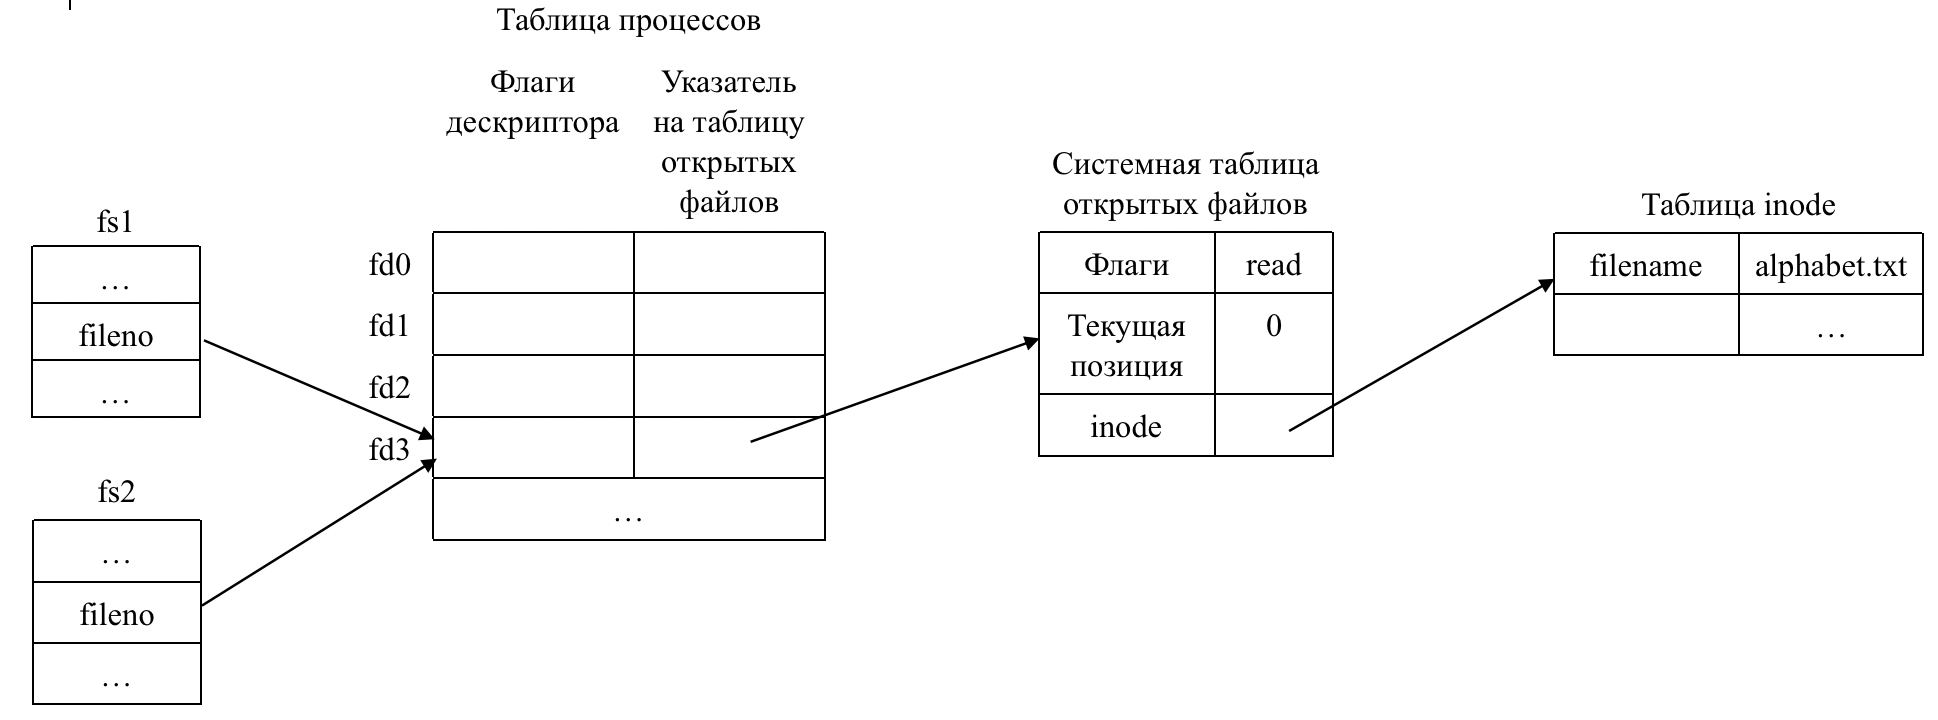
\includegraphics[scale=0.6]{shema1}

\newpage

\textbf{Задание 2:} Проанализировать работу приведенной программы и объяснить результат ее работы. 

\begin{lstlisting}[]
#include <fcntl.h>
#include <unistd.h>
#include <errno.h>
#include <string.h>
#include <stdio.h>

int main()
{
  // Создает файловый дескриптор для открытого файла 2 раза
  int fd1 = open("alphabet.txt", O_RDONLY);
  if (fd1 == -1)
  {
    printf("%s", strerror(errno));
    return errno;
  }

  int fd2 = open("alphabet.txt", O_RDONLY);
  if (fd2 == -1)
  {
    printf("%s", strerror(errno));
    return errno;
  }

  // Чтение char и вывод на экран попеременно
  char c1;
  char c2;
  // read возвращает количество действительно считанных байт.
  // Соответственно, когда кол-во считанных байтов не будет равно 1,
  // значит или конец файла или ошибка.
  while ((read(fd1, &c1, 1) == 1) && (read(fd2, &c2, 1) == 1))
  {
    write(1, &c1, 1);
    write(1, &c2, 1);
  }

  close(fd1);
  close(fd2);

  return 0;
}
\end{lstlisting}

\textbf{Результат:}


\includegraphics[scale=0.9]{2}

При использовании системного вызова open() создаются 2 разных файловых дескриптора для открытого файла, 2 записи в общесистемной таблице открытых файлов. 

Файловые дескрипторы разные, поэтому у каждого своя текущая позиция файла.

Тогда с помощью системных вызовов read(), write() в результате получится строка с дублирующимися символами. 

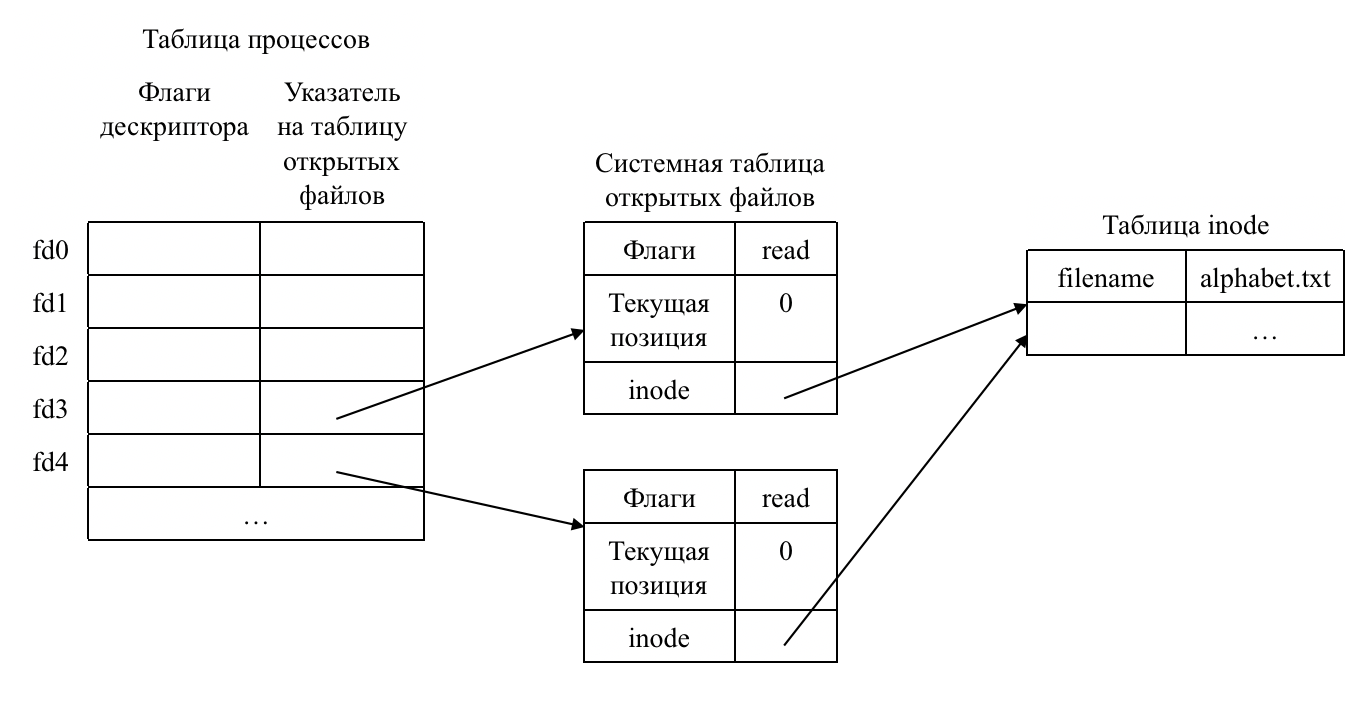
\includegraphics[scale=0.7]{shema2}

\newpage

\textbf{Задание 3:} Написать программу, которая открывает один и тот же файл два раза с использованием библиотечной функции fopen(). Для этого объявляются два файловых дескриптора. В цикле записать в файл буквы латинского алфавита поочередно передавая функции fprintf() то первый дескриптор, то – второй.
Результат прокомментировать.

\begin{lstlisting}[]
#include <fcntl.h>
#include <stdio.h>
#include <errno.h>
#include <string.h>

int main()
{
  // Открывает файл и связывает с ним буферизованный поток
  FILE *fd1 = fopen("test3.txt", "w");
  if (fd1 == NULL)
  {
    printf("%s", strerror(errno));
    return errno;
  }

  FILE *fd2 = fopen("test3.txt", "w");
  if (fd1 == NULL)
  {
    printf("%s", strerror(errno));
    return errno;
  }

  // Цикл по всем буквам алфавита (нечетные - fd1, четные - fd2)
  for(char c = 'a'; c <= 'z'; c++)
  {
    if (c % 2)
    {
      fprintf(fd1, "%c", c);
    }
    else
    {
      fprintf(fd2, "%c", c);
    }
  }

  fclose(fd1);
  fclose(fd2);
  return 0;
}
\end{lstlisting}

\textbf{Результат:}

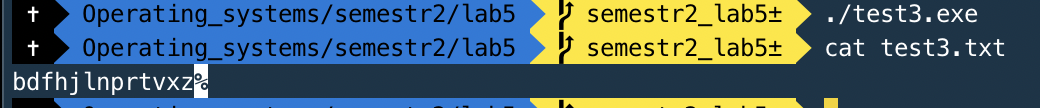
\includegraphics[scale=0.9]{3}

При вызове функции fopen() 2 раза с аргументом <<w>> (открытие для записи) создаются 2 разных файловых дескриптора файла и две независимые позиции в файле указывают на начало. 

В цикле с использованием функции fprintf в буферизованные потоки записываются буквы от a до z, нечетные в первый поток (a, c, e...), а четные во второй (b, d, f ...). Поскольку используются различные дескрипторы, то смещение текущей позиции файла при каждом вызове fprintf() происходит независимо.

Так как fprintf() обеспечивает буферизованный вывод -- запись непосредственно в файл осуществляется только при вызове функции fclose(), fflush(), либо при полном заполнении буфера.

Функция fclose(fd1) очистит поток, на который указывает fd1(запись любых буферизованных выходных данных с помощью fflush (принудительно записывает все буферизированные данные в устройство вывода данных)), и закроет файловый дескриптор.

Далее вызывается fclose(fd2), так как оба потока открыты открыты на запись в файл, то после его выполнения данные в файле, записанные с помощью первого потока, перезапишутся данными из второго потока. 

\hfill

Если хотим, чтобы в файл можно было добавлять данные с помощью двух независимых дескрипторов (без опасения нарушить вывод), то необходимо открыть файл в режиме добавления с аргументом <<а>>, тогда все последующие операции записи в файл будут работать с current end-of-file. 

Информация будет записана в файл в том порядке, в котором процессы записывали ее в файл (запись непосредственно в файл осуществляется только при вызове функции fclose(), fflush(), либо при полном заполнении буфера).

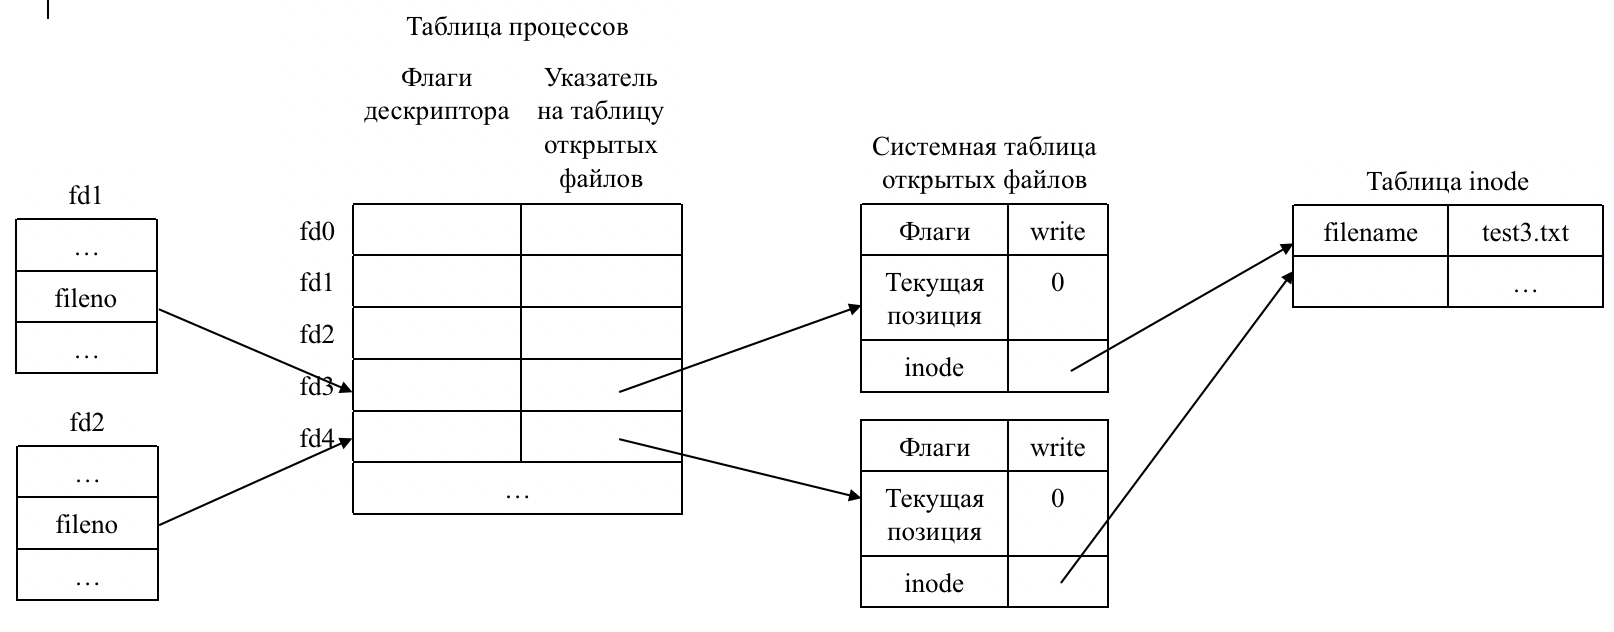
\includegraphics[scale=0.6]{shema3}

\newpage

\textbf{struct FILE} 

\begin{lstlisting}
typedef struct __sFILE {
    unsigned char *_p;	/* current position in (some) buffer */
    int	_r;		/* read space left for getc() */
    int	_w;		/* write space left for putc() */
    short _flags;	/* flags, below; this FILE is free if 0 */
    short _file;	/* fileno, if Unix descriptor, else -1 */
    struct __sbuf _bf;	/* the buffer (at least 1 byte, if !NULL) */
    int	_lbfsize;	/* 0 or -_bf._size, for inline putc */

    /* operations */
    void *_cookie;	/* cookie passed to io functions */
    int	(* _Nullable _close)(void *);
    int	(* _Nullable _read) (void *, char *, int);
    fpos_t	(* _Nullable _seek) (void *, fpos_t, int);
    int	(* _Nullable _write)(void *, const char *, int);

    /* separate buffer for long sequences of ungetc() */
    struct __sbuf _ub;       /* ungetc buffer */
    struct __sFILEX *_extra; /* additions to FILE to not break ABI */
    int	_ur;		     /* saved _r when _r is counting ungetc data */

    /* tricks to meet minimum requirements even when malloc() fails */
    unsigned char _ubuf[3];	/* guarantee an ungetc() buffer */
    unsigned char _nbuf[1];	/* guarantee a getc() buffer */

    /* separate buffer for fgetln() when line crosses buffer boundary */
    struct	__sbuf _lb;	/* buffer for fgetln() */

    /* Unix stdio files get aligned to block boundaries on fseek() */
    int	_blksize;	/* stat.st_blksize (may be != _bf._size) */
    fpos_t _offset;	/* current lseek offset (see WARNING) */
} FILE;
\end{lstlisting}

Функция fileno(FILE *stream) возвращает целочисленный файловый дескриптор, связанный с потоком, на который указывает stream.

\end{document}